\documentclass[12pt,a4paper]{article}
 
\usepackage{float}
%für feststellen der figures und tables [H] dranschreiben
\usepackage{units}
%wird so benutzt: 
%\unit[value/Zahl]{dimension/Einheit} oder 
%\unitfrac[value/Zahl]{dimension/Einheit num/Zähler}{dimension/Einheit denum/Nenner} oder
%\nicefrac[fontcommand/Schriftart]{dimension/Einheit num/Zähler}{dimension/Einheit denum/Nenner}
\usepackage{amssymb}
\usepackage{caption}
\usepackage{subcaption}

\usepackage{hyperref}

\usepackage[left=2cm,right=2cm,top=2cm,bottom=2cm]{geometry}
\usepackage[utf8]{inputenc}
\usepackage[T1]{fontenc}
\usepackage{lmodern}
\usepackage[ngerman]{babel}
\usepackage{amsmath}
\usepackage{graphicx}
 
%niemals zwei überschriften direkt übereinander schreiben, also immer mindestens in einem satz was sinnvolles unter jede überschrift schreiben (bei den versuchen z.B. das versuchsziel) 
\begin{document}
%deckblatt erstellen.


\begin{titlepage}

\begin{center}
% Oberer Teil der Titelseite:

\includegraphics[width=0.75\textwidth]{logo.pdf}\\[1cm]    	%Logo 

\textsc{\LARGE Bergische Universität Wuppertal}\\[1.5cm]	%Institution

\textsc{\Large Elektronik Praktikum}\\[0.5cm]				%Projekt


\newcommand{\HRule}{\rule{\linewidth}{0.5mm}}
\HRule \\[0.4cm]
{ \huge \bfseries Datenerfassung mit dem Computer}\\[0.4cm]				%Titel

\HRule \\[1.5cm]

% Author und Tutor
\begin{minipage}{0.4\textwidth}
\begin{flushleft} \large
\emph{Verfasser:}\\
Henrik \textsc{Jürgens} \\
Frederik \textsc{Strothmann}
\end{flushleft}
\end{minipage}
\hfill
\begin{minipage}{0.4\textwidth}
\begin{flushright} \large
\emph{Tutoren:} \\
Hans-Peter \textsc{Kind} \\
Peter \textsc{Knieling} \\
Marius \textsc{Wensing}
\end{flushright}
\end{minipage}

\vfill

% Unterer Teil der Seite/Datum
{\large \today}

\end{center}

\end{titlepage}

\newpage
\tableofcontents
\newpage
\section{Einleitung}
%einleitung zu dem experiment.
%auf die einstellungen, die vor dem versuch gemacht werden, eingehen oder auf eine anleitung dazu verweisen
%es soll immer erwähnt werden um was es in dem Versuch geht und wie das relisiert werden soll
%---------------------------------------------------------------------------------------------
%hinter der einleitung kann der allgemeine theoretische hintergrund in einer zusätzlichen section erklärt werden
%1-----------------------------------------------1

Dieser Versuch beschäftigt sich mit den Fragestellungen, wie man digitale in analoge Signale umwandelt, wie ein Computer kontinuierliche Spannungswerte erzeugen kann, wie analoge Werte digitalisiert werden können, wie ein Digitalvoltmeter kontinuierliche Spannungswerte erfassen, digital anzeigen kann und wie sich Zeiten oder Frequenzen messen lassen.

\section{Umwandlung digitaler in analoge Signale, DAC}
%kurz das ziel dieses versuchsteiles ansprechen, damit keine zwei überschriften direkt übereinander stehen!
%bei schwierigeren versuchen kann auch der theoretische hintergrund erläutert werden. (mit formeln, herleitungen und erklärungen)

In diesem Versuchsabschnitt werden verschiedene Digital-Analog-Converter gebaut und untersucht. Realisiert werden ein Digital-Analog-Converter mit Binär- und R-2R-Netzwerk. 

\subsection{DAC mit binärem Netzwerk}
%kurz das ziel dieses versuchsteiles ansprechen, damit keine zwei überschriften direkt übereinander stehen!
%bei schwierigeren versuchen kann auch der theoretische hintergrund erläutert werden. (mit formeln, herleitungen und erklärungen)

In diesem Versuchsteil wird ein DAC mit einem Binärnetzwerk aufgebaut. Der Nachteil dieses Aufbaus ist, dass für hohe Auflösungen genaue Widerstände benötigt werden. Die Ausgangsspannung bestimmt sich mit:
\begin{align}
\text{U}_\text{A}=\text{U}_0 \cdot \frac{\text{Binärwert}}{2^\text{n}-1}
\label{eqn:binaer}
\end{align}

Dabei ist n die Bitgröße des Eingangssignals.

\subsubsection*{Verwendete Geräte}
%(immer) eine skizze oder ein foto einfügen, die geräte/materialien !nummerieren! und z.b. eine legende dazu schreiben, besser wäre es das ganze in einem Fließtext gut zu beschreiben.
%falls am anfang des versuches nicht klar ist, was alles verwendet wird, wenn möglich erst am ende ein großes foto von den verwendeten materialien machen!\\

Es werden das Versuchsboard, das Zusatzboard, ein PC, ein Steckaufsatz und n Widerstände der Größe $2^\text{j}$ (j=1$,\ldots$,n) verwendet.

\subsubsection*{Versuchsaufbau} 
%skizze zum versuchsaufbau (oder foto) einfügen,   es muss erklärt werden wie das ganze funktioniert und welche speziellen einstellungen verwendet wurden (z.b. welche knöpfe an den geräten für die messung verdreht wurden)

In Abbildung \ref{fig:auf_1_1} ist der Schaltplan eines ADCs mit binärem Widerstandsnetzwerk zu sehen. Die Schaltung wird mit dem Versuchsboard und einem Binärnetzwerk realisiert.

\begin{figure}[H] 
  \centering 	
    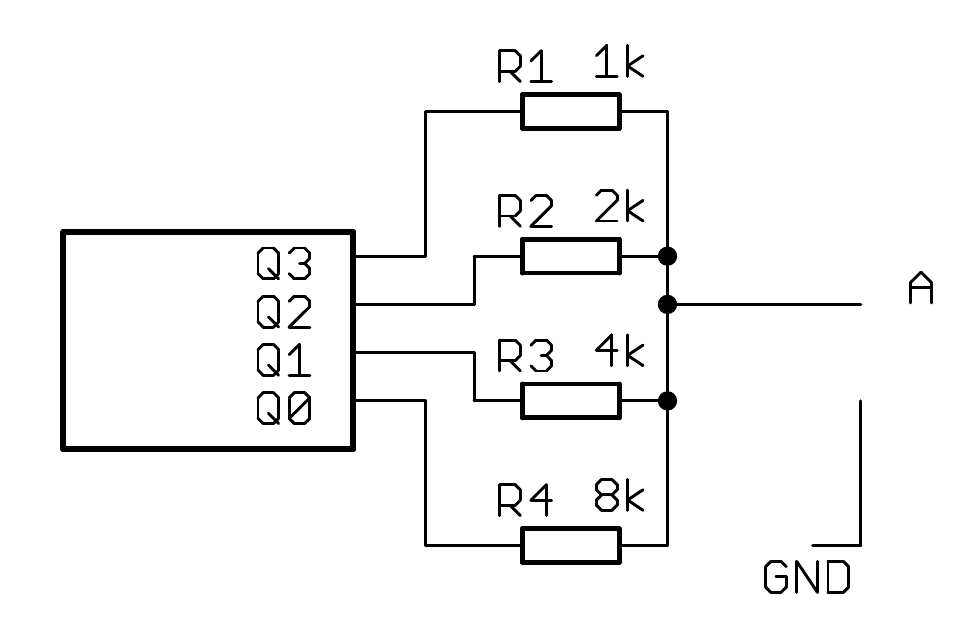
\includegraphics[ scale = 0.4]{auf_1_1.png}
  	\caption[Schaltplan für ein DAC mit binärem Widerstandsnetzwerk]{Schaltplan für ein DAC mit binärem Widerstandsnetzwerk\footnotemark}
  \label{fig:auf_1_1}
\end{figure}
\footnotetext{Abbildung entnommen von http://www.atlas.uni-wuppertal.de/$\sim$kind/ep11\_14.pdf am 18.01.2015}

\subsubsection*{Versuchsdurchführung}
%erklären, !was! wir machen, !warum! wir das machen und mit welchem ziel
%(wichtig) präzize erklären, wie bei dem versuch vorgegangen und was gemacht wurde

Der größte Widerstand (1,3M$\Omega$) wird an die erste Binärstelle angeschlossen und an jede weitere Binärstelle jeweils die Hälfte des vorherigen Widerstandes. Das Widerstandsnetzwerk wird auf das Versuchsboard gesteckt. Zuerst werden die ersten 4 Bits, danach die ersten 8 Bits verwendet und mit dem Oszilloskop das Ausgangssignal aufgenommen. Die Messung wird mit dem Befehl c gestartet. Der Mikrocontroller übernimmt in diesem Fall die Funktionen des Oszillators und des Binärzählers.

\subsubsection*{Auswertung}
%zuerst !alle! errechneten werte entweder in ganzen sätzen aufzählen, oder in tabellen (übersichtlicher) dargestellen, sowie auf die verwendeten formeln verweisen (die referenzierung der formel kann in der überschrift stehen)
%kurz erwähnen (vor der tabelle), warum wir das ganze ausrechnen bzw. was wir dort ausrechnen
%danach histogramme und plots erstellen, wobei wenn möglich funktionen durch die plots gelegt werden (zur not können auch splines benutzt werden, was aber angegeben werden muss)
%bei fits immer die funktion und das reduzierte chiquadrat mit angegeben, wobei auf verständlichkeit beim entziffern der zehnerpotenzen geachtet werden muss z.b. f(x)=(wert+-fehler)\cdot10^{irgendeine zahl}\cdot x + (wert+-fehler)\cdot10^{irgendeine zahl}
%bei jedem fit erklären, nach welchem zusammenhang gefittet wurde und warum!
%bei plots darauf achten, dass die achsenbeschriftung (auch die tics) die richtige größe haben und die legende im plot nicht die messwerte verdeckt
%kurz die aufgabenstellung abhandeln
%2-----------------------------------------------2

Bei der Messung wird ein treppen-artiger Verlauf der Ausgangsspannung erwartet. Die Differenz zwischen zwei Stufen ergibt sich nach Gleichung \ref{eqn:binaer} mit $\frac{\text{U}_0}{2^\text{n}-1}$. Für die 4 Bits ergab sich der Verlauf in Abbildung \ref{fig:1_1_1}, die einzelnen Stufen sind deutlich zu sehen. Die Auflösung liegt bei einem fünfzentel.

\begin{figure}[H] 
  \centering 	
    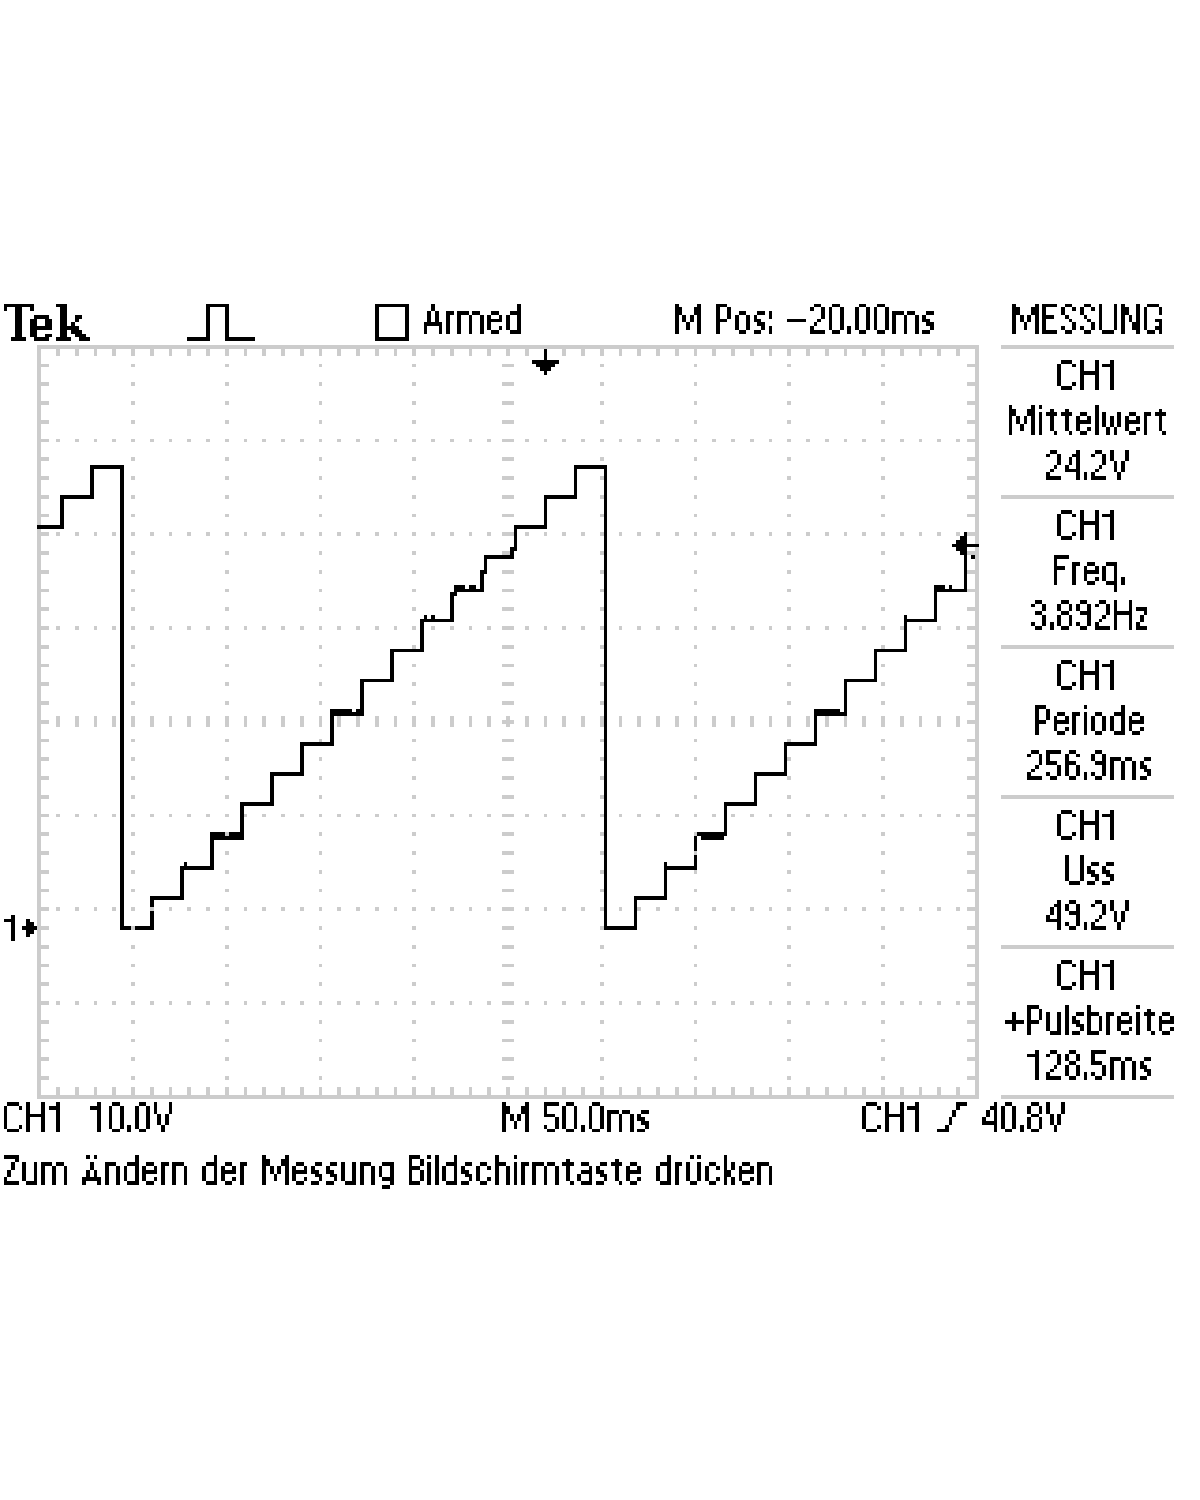
\includegraphics[trim = 0mm 50mm 0mm 50mm, clip, scale = 0.4]{1_1_1.pdf}
  	\caption[Aufnahme der Ausgangsspannung mit 4 Widerständen]{Aufnahme der Ausgangsspannung mit 4 Widerständen} 
  \label{fig:1_1_1}
\end{figure}

Die Aufnahme des Kurvenverlaufs für 8 Bit ist in Abbildung \ref{fig:1_1_2} zu sehen. Die Stufen sind nicht zu erkennen, dies liegt an der Auflösung, die bei einem 255-stel liegt.

\begin{figure}[H] 
  \centering 	
    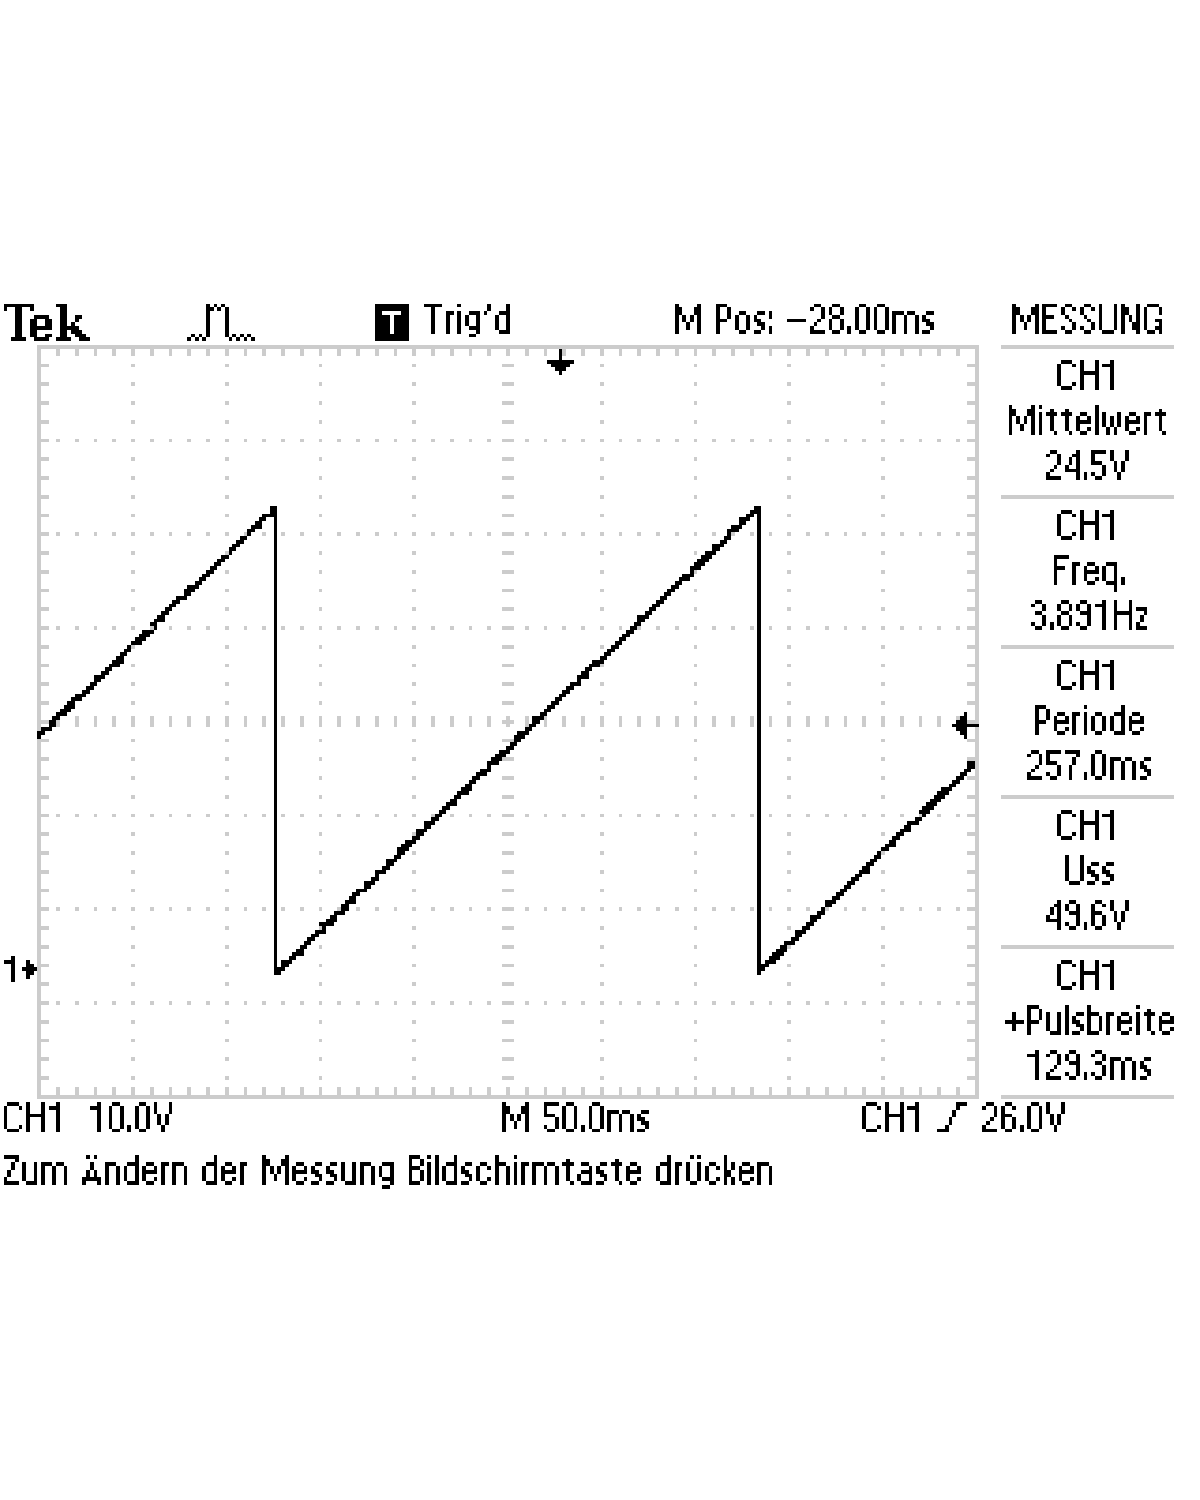
\includegraphics[trim = 0mm 50mm 0mm 50mm, clip, scale = 0.4]{1_1_2.pdf}
  	\caption[Aufnahme der Ausgangsspannung mit 8 Widerständen]{Aufnahme der Ausgangsspannung mit 8 Widerständen} 
  \label{fig:1_1_2}
\end{figure}



\subsection{DAC mit R-2R-Netzwerk}
%kurz das ziel dieses versuchsteiles ansprechen, damit keine zwei überschriften direkt übereinander stehen!
%bei schwierigeren versuchen kann auch der theoretische hintergrund erläutert werden. (mit formeln, herleitungen und erklärungen)

In diesem Versuchsteil wird ein DAC mit einem R-2R-Netzwerk untersucht. Der Vorteil dieses Aufbaus ist, dass nur zwei verschiedene Widerstände benötigt werden, die ein Verhältnis von 1:2 haben. Die Auflösung bestimmt sich mit:

\begin{align}
\text{U}_\text{A}=\text{U}_0 \cdot \frac{\text{Binärwert}}{2^\text{n}}
\label{eqn:binaer_2}
\end{align}

\subsubsection*{Verwendete Geräte}
%(immer) eine skizze oder ein foto einfügen, die geräte/materialien !nummerieren! und z.b. eine legende dazu schreiben, besser wäre es das ganze in einem Fließtext gut zu beschreiben.
%falls am anfang des versuches nicht klar ist, was alles verwendet wird, wenn möglich erst am ende ein großes foto von den verwendeten materialien machen!\\

Es werden das Versuchsboard, das Zusatzboard, ein PC und ein Steckaufsatz mit einem R-2R Widerstandsnetzwerk verwendet.

\subsubsection*{Versuchsaufbau}
%skizze zum versuchsaufbau (oder foto) einfügen,   es muss erklärt werden wie das ganze funktioniert und welche speziellen einstellungen verwendet wurden (z.b. welche knöpfe an den geräten für die messung verdreht wurden)

Der Schaltplan eines R-2R Netzwerkes ist in Abbildung \ref{fig:auf_1_2} zu sehen. Dieses Netzwerk wird auf das Zusatzboard gesetzt.

\begin{figure}[H] 
  \centering
    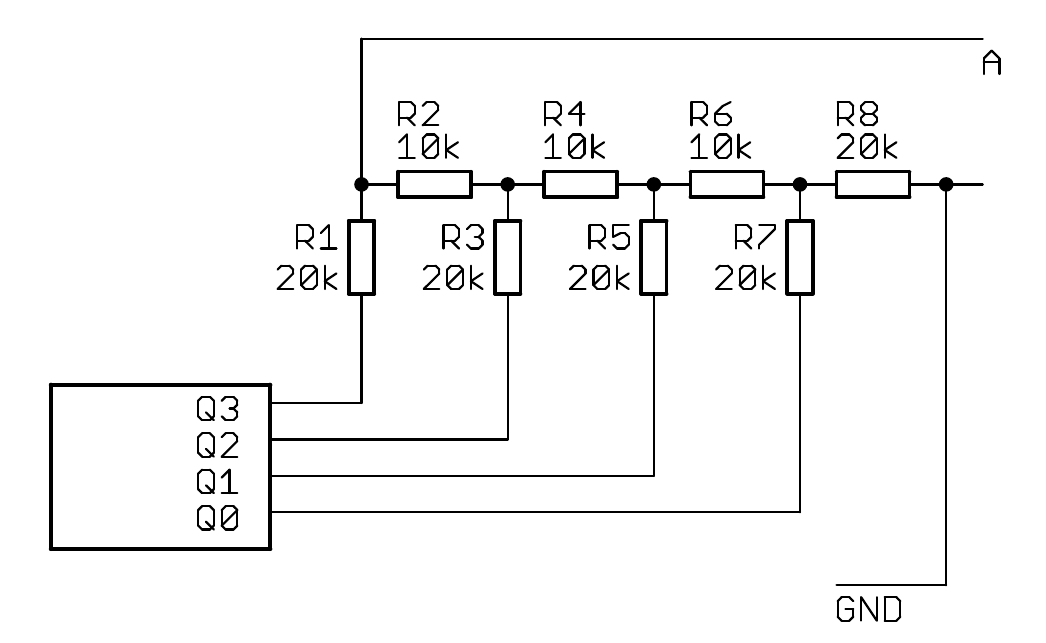
\includegraphics[ scale = 0.4]{auf_1_2.png}
  	\caption[Schaltplan für einen R-2R Netzwerk]{Schaltplan für einen R-2R Netzwerk\footnotemark}
  \label{fig:auf_1_2}
\end{figure}
\footnotetext{Abbildung entnommen von http://www.atlas.uni-wuppertal.de/$\sim$kind/ep11\_14.pdf am 18.01.2015}

\subsubsection*{Versuchsdurchführung}
%erklären, !was! wir machen, !warum! wir das machen und mit welchem ziel
%(wichtig) präzize erklären, wie bei dem versuch vorgegangen und was gemacht wurde

Das für acht Bit ausgelegte R-2R-Netzwerk wird auf das Versuchsboard gesteckt. Die Messung wird mit dem Befehl c gestartet und das Ausgangssignal mit dem Oszilloskop  untersucht.

\subsubsection*{Auswertung}
%zuerst !alle! errechneten werte entweder in ganzen sätzen aufzählen, oder in tabellen (übersichtlicher) dargestellen, sowie auf die verwendeten formeln verweisen (die referenzierung der formel kann in der überschrift stehen)
%kurz erwähnen (vor der tabelle), warum wir das ganze ausrechnen bzw. was wir dort ausrechnen
%danach histogramme und plots erstellen, wobei wenn möglich funktionen durch die plots gelegt werden (zur not können auch splines benutzt werden, was aber angegeben werden muss)
%bei fits immer die funktion und das reduzierte chiquadrat mit angegeben, wobei auf verständlichkeit beim entziffern der zehnerpotenzen geachtet werden muss z.b. f(x)=(wert+-fehler)\cdot10^{irgendeine zahl}\cdot x + (wert+-fehler)\cdot10^{irgendeine zahl}
%bei jedem fit erklären, nach welchem zusammenhang gefittet wurde und warum!
%bei plots darauf achten, dass die achsenbeschriftung (auch die tics) die richtige größe haben und die legende im plot nicht die messwerte verdeckt
%kurz die aufgabenstellung abhandeln
%2-----------------------------------------------2

Für den zeitlichen Verlauf wird ein Treppen-artiger Verlauf erwartet. Dabei ist die Auflösung höher, da die Ausgangsspannung nach Gleichung \ref{eqn:binaer_2} bestimmt wird. Die Höhe einer Stufe ergibt sich mit $\frac{\text{U}_0}{2^\text{n}}$. In dem verwendeten Aufbau entspricht dies einer Stufenhöhe von einem 256-stel. Der Verlauf auf dem Oszilloskop ist in Abbildung \ref{fig:1_2_1} zu sehen. Aufgrund der hohen Auflösung sind die einzelnen Stufen nicht mehr zu erkennen.

\begin{figure}[H] 
  \centering 	
    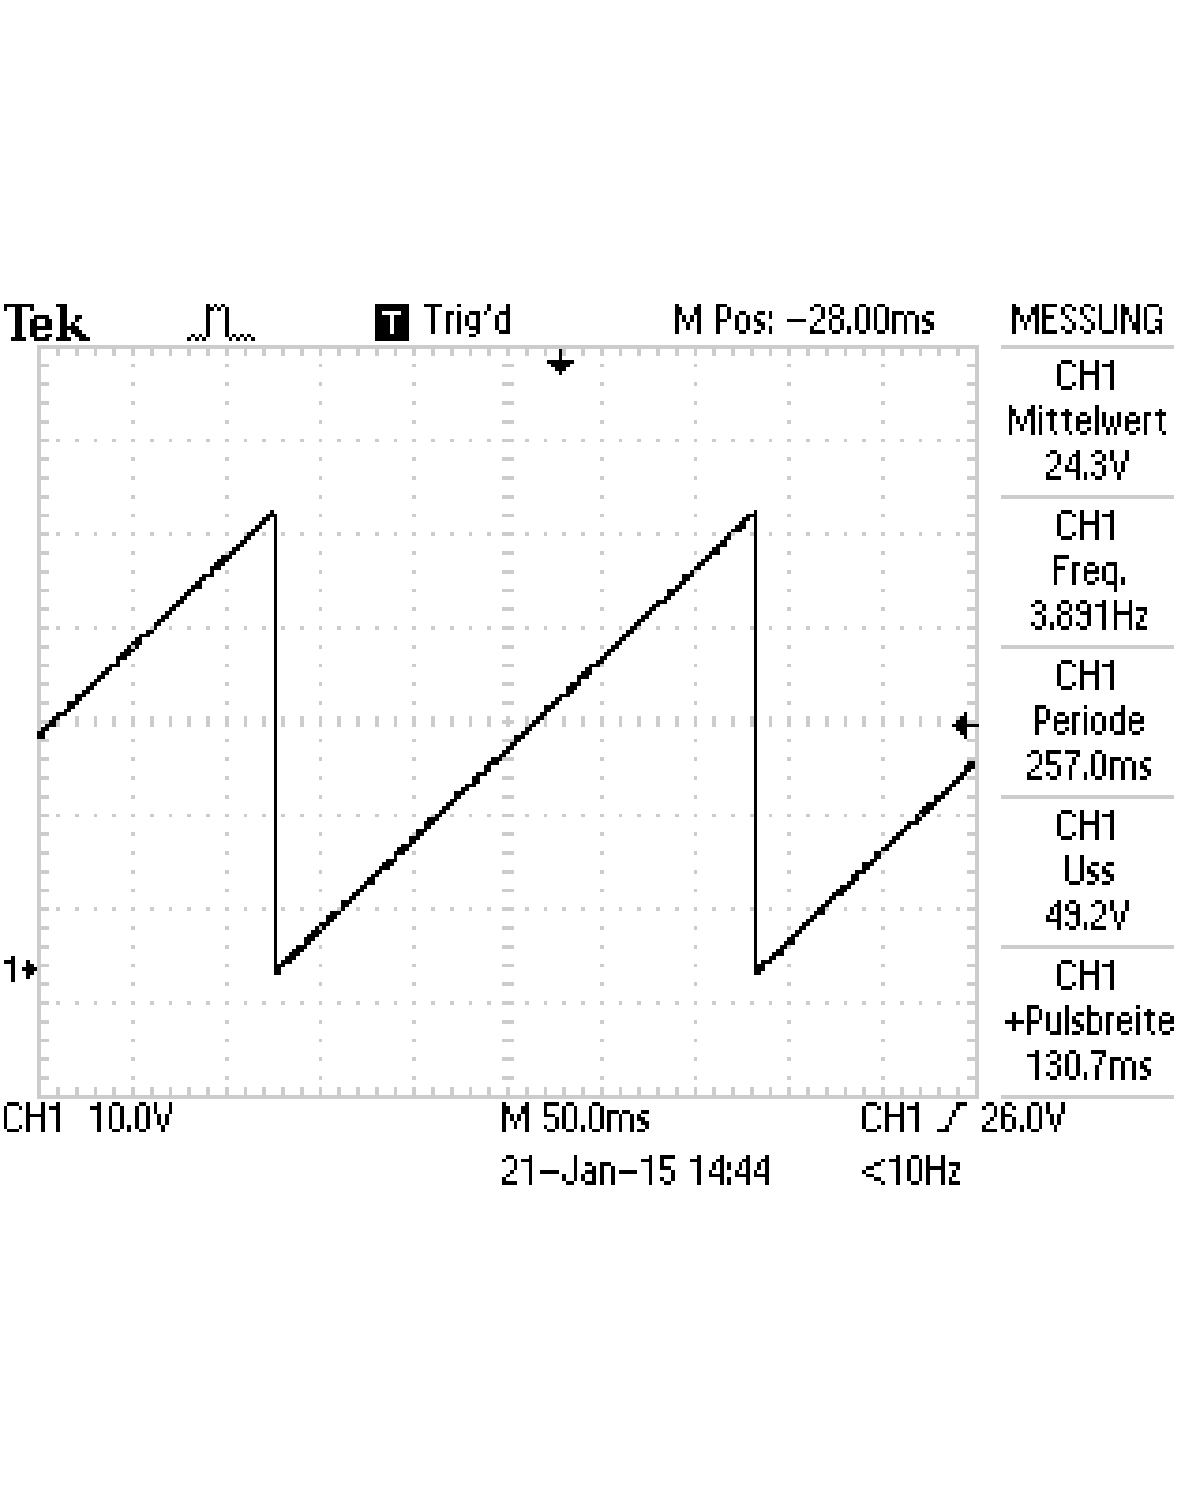
\includegraphics[trim = 0mm 50mm 0mm 50mm, clip, scale = 0.4]{1_2_1.pdf}
  	\caption[Aufnahme der Ausgangsspannung]{Aufnahme der Ausgangsspannung} 
  \label{fig:1_2_1}
\end{figure}
 

\subsubsection*{Diskussion}
%(immer) die gemessenen werte und die bestimmten werte über die messfehler mit literaturwerten oder untereinander vergleichen
%in welchem fehlerintervall des messwertes liegt der literaturwert oder der vergleichswert?
%wie ist der relative anteil des fehlers am messwert und damit die qualität unserer messung?
%in einem satz erklären, wie gut unser fehler und damit unsere messung ist
%kurz erläutern, wie systematische fehler unsere messung beeinflusst haben könnten
%(wichtig) zum schluss ansprechen, in wie weit die ergebnisse mit der theoretischen vorhersage übereinstimmen
%--------------------------------------------------------------------------------------------
%falls tabellen mit den messwerten zu lang werden, kann die section mit den messwerten auch hinter der diskussion angefügt bzw. eine section mit dem anhang eingefügt werden.
%1-----------------------------------------------1

Beide Messungen sind wie erwartet verlaufen. Da für das R-2R Netzwerk nur ein 8 Bit großes Netzwerk zur Verfügung stand, können nur die beiden 8 Bit großen ADC verglichen werden. Betrachtet man die beiden Aufnahmen, Abbildung \ref{fig:1_1_2} für das Binärnetzwerk und Abbildung \ref{fig:1_2_1} für das R-2R Netzwerk, ist kein Unterschied zu erkennen. Theoretisch sollten sich mit dem R-2R Netzwerk bessere Ergebnisse erzielen lassen, da es kaum von den Fehlern der Widerstände abhängt.



\section{Umwandlung analoger in digitale Signale, ADC}
%kurz das ziel dieses versuchsteiles ansprechen, damit keine zwei überschriften direkt übereinander stehen!
%bei schwierigeren versuchen kann auch der theoretische hintergrund erläutert werden. (mit formeln, herleitungen und erklärungen)

In diesem Versuchsabschnitt werden verschiedene Analog-Digital-Converter mit Hilfe des Boards aus Versuch 10 gebaut.

\subsection{ADC mit Zählverfahren und mit Approximationsverfahren}
%kurz das ziel dieses versuchsteiles ansprechen, damit keine zwei überschriften direkt übereinander stehen!
%bei schwierigeren versuchen kann auch der theoretische hintergrund erläutert werden. (mit formeln, herleitungen und erklärungen)

In diesem Versuchsteil wird ein ADC mit Zählverfahren und ein ADC mit Apporximatoinsverfahren gebaut.

Der ADC mit Zählverfahren verwendet einen Binärzähler und ein R-2R Netzwerk um die Referenzspannung zu erzeugen. Der Stand des Binärzählers wird gespeichert, wenn der Komparator eine 0 ausgibt. Das Bitmuster des Zählers entspricht der digitalen Version des analogen Signals. Der Nachteil des Verfahrens ist, dass der Aufwand zur Digitalisierung des Signals $\mathcal O(2^n)$ beträgt.

Der ADC mit Apporximatoinsverfahren besteht aus einer Steuereinheit, einem R-2R Netzwerk und einem Komparator. Die Steuereinheit schaltet die Referenzspannung auf den halben Maximalwert. Wenn der Ausgang des Komparators auf 1 eins geht, wird die Referenzspannung auf $\frac{3}{4}$ der Maximalspannung gesetzt. Falls der Ausgang des Komparators auf 0 steht wird das aktuelle Bit auf 0 gesetzt und die Referenzspannung auf $\frac{1}{4}$ der Maximalspannung gesetzt. Der Vorteil dieses Verfahren ist, dass es wesentlich schneller als das Zählverfahren ist. Der Aufwand beträgt $\mathcal O(n)$.

\subsubsection*{Verwendete Geräte}
%(immer) eine skizze oder ein foto einfügen, die geräte/materialien !nummerieren! und z.b. eine legende dazu schreiben, besser wäre es das ganze in einem Fließtext gut zu beschreiben.
%falls am anfang des versuches nicht klar ist, was alles verwendet wird, wenn möglich erst am ende ein großes foto von den verwendeten materialien machen!\\

Es werden das Board aus Versuch 10, ein Zusatzboard, ein Oszilloskop und ein Netzgerät verwendet.


\subsubsection*{Versuchsaufbau}
%skizze zum versuchsaufbau (oder foto) einfügen,   es muss erklärt werden wie das ganze funktioniert und welche speziellen einstellungen verwendet wurden (z.b. welche knöpfe an den geräten für die messung verdreht wurden)

Der Versuchsaufbau besteht aus dem Board von Versuch 10 und einem neuem Zusatzboard, in dem alle notwendigen Komponenten integriert sind.

\begin{figure}[H] 
  \centering 	
    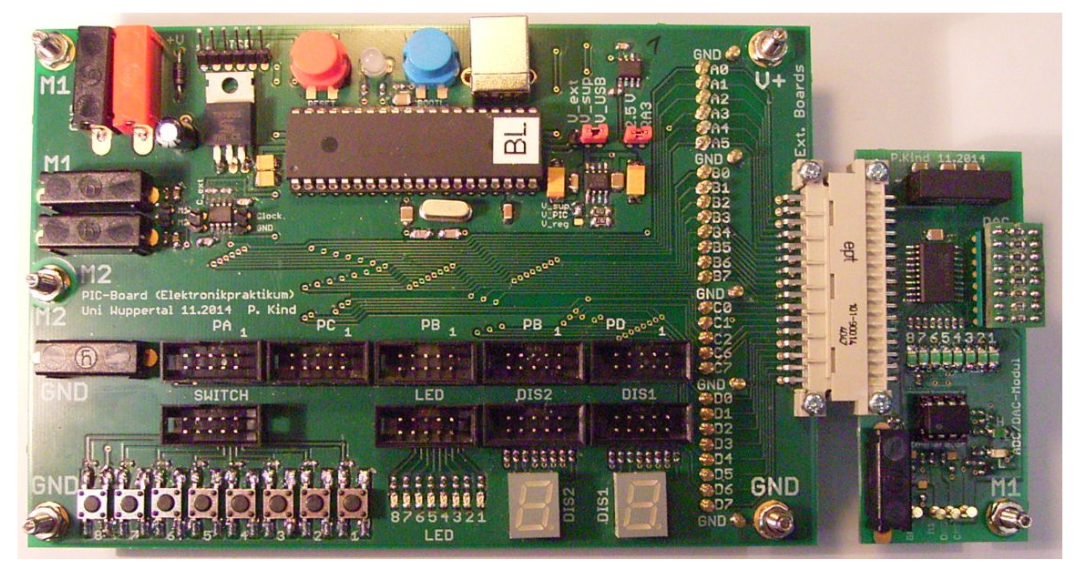
\includegraphics[ scale = 0.4]{auf_4.png}
  	\caption[Board und Zusatzborad]{Board und Zusatzborad\footnotemark}
  \label{fig:auf_2}
\end{figure}
\footnotetext{Abbildung entnommen von http://www.atlas.uni-wuppertal.de/$\sim$kind/ep11\_14.pdf am 18.01.2015}

\subsubsection*{Versuchsdurchführung}
%erklären, !was! wir machen, !warum! wir das machen und mit welchem ziel
%(wichtig) präzize erklären, wie bei dem versuch vorgegangen und was gemacht wurde

Das Zusatzboard wird an das Board angeschlossen, dies geschieht über einen seriellen Anschluss. Das vorgeschriebene Programm, zum messen der Daten wird auf das Board geladen. Danach wird die zu messende Spannung an M1 angeschlossen. Die Funktionalität wird untersucht, indem verschiedene Steuerzeichen (siehe nachfolgende Tabelle) an den Mikrocontroller geschickt werden. Dann werden unterschiedliche Spannungen eingestellt und die Ausgangssignale mit dem Oszilloskop beobachtet. Das Bitmuster wird jeweils abgelesen und notiert. Der Vorgang wird für das Zählverfahren und das Approximationsverfahren durchgeführt. Im nachfolgenden ist die Tabelle mit den Befehlen zu sehen.

\begin{itemize}
\item	?: Mikrocontroller meldet E-Prak Bergische Universität Wuppertal 2011“

\item	v: Mikrocontroller meldet Versionsnummer des Programms (V. PIC-Eval-Board for EP 1.2011)

\item	t: Mikrocontroller meldet OK“(Test der Verbindung)

\item	i: Mikrocontroller führt eine Messung nach dem Zählverfahren aus (iterativ, 10 ms Verzögerung)

\item	s: Mikrocontroller führt eine Messung nach dem Approximationsverfahren aus (sukzessiv, 10 ms Verzögerung)

\item	a: Mikrocontroller führt eine Messung nach dem Approximationsverfahren aus (sukzessiv durch Tasterfunktion an Port A0 mit 300 ms Verzögerung zum Entprellen)

\item	bxx: Gibt das Binärmuster xx (xx= hexadezimale Zahl von 00 bis ff) am Port B aus. Zum Beispiel b00 liefert 00000000, b01 liefert 00000001, b0f liefert 00001111 und bff liefert 11111111

\end{itemize}

\subsubsection*{Messwerte}

Messdaten für das Zählverfahren.

\begin{table}[htbp]
\begin{center}
\begin{tabular}{|c|c|c|c|c|}
\hline
\multicolumn{1}{|l|}{Spannung/V} & Hex & \multicolumn{1}{l|}{Decimal} & \multicolumn{1}{l|}{Erwartet Binärwerte} & LEDs \\ \hline
0,5 & 1E & 30 & 0b00011110 & 0b00011110 \\ \hline
1 & 39 & 57 & 0b00111001 & 0b00111001 \\ \hline
1,5 & 55 & 85 & 0b01010101 & 0b01010101 \\ \hline
2 & 6F & 111 & 0b01101111 & 0b01101111 \\ \hline
2,5 & 89 & 137 & 0b10001001 & 0b10001001 \\ \hline
3 & A3 & 163 & 0b10100011 & 0b10100011 \\ \hline
3,5 & BD & 189 & 0b10111101 & 0b10111101 \\ \hline
4 & D5 & 213 & 0b11010101 & 0b11010101 \\ \hline
4,5 & EF & 239 & 0b11101111 & 0b11101111 \\ \hline
5 & FF & 255 & 0b11111111 & 0b11111111 \\ \hline
\end{tabular}
\end{center}
\caption{Messung zum Zählverfahren}
\label{tab:zaehl}
\end{table}

Messdaten für das Approximationsverfahren.

\begin{table}[htbp]
\begin{center}
\begin{tabular}{|c|c|c|c|c|}
\hline
\multicolumn{1}{|l|}{Spannung/V} & Hex & \multicolumn{1}{l|}{Decimal} & \multicolumn{1}{l|}{Erwartet Binärwerte} & LEDs \\ \hline
0,5 & 1F & 31 & 0b00011111 & 0b00011111 \\ \hline
1 & 38 & 56 & 0b00111000 & 0b00111000 \\ \hline
1,5 & 4F & 79 & 0b01001111 & 0b01001111 \\ \hline
2 & 6F & 111 & 0b01101111 & 0b01101111 \\ \hline
2,5 & 87 & 135 & 0b10000111 & 0b10000111 \\ \hline
3 & A0 & 160 & 0b10100000 & 0b10100000 \\ \hline
3,5 & BE & 190 & 0b10111110 & 0b10111110 \\ \hline
4 & D8 & 216 & 0b11011000 & 0b11011000 \\ \hline
4,5 & EF & 239 & 0b11101111 & 0b11101111 \\ \hline
5 & FF & 255 & 0b11111111 & 0b11111111 \\ \hline
\end{tabular}
\end{center}
\caption{Messung zum Approximationsverfahren}
\label{tab:approx}
\end{table}



\subsubsection*{Auswertung}
%zuerst !alle! errechneten werte entweder in ganzen sätzen aufzählen, oder in tabellen (übersichtlicher) dargestellen, sowie auf die verwendeten formeln verweisen (die referenzierung der formel kann in der überschrift stehen)
%kurz erwähnen (vor der tabelle), warum wir das ganze ausrechnen bzw. was wir dort ausrechnen
%danach histogramme und plots erstellen, wobei wenn möglich funktionen durch die plots gelegt werden (zur not können auch splines benutzt werden, was aber angegeben werden muss)
%bei fits immer die funktion und das reduzierte chiquadrat mit angegeben, wobei auf verständlichkeit beim entziffern der zehnerpotenzen geachtet werden muss z.b. f(x)=(wert+-fehler)\cdot10^{irgendeine zahl}\cdot x + (wert+-fehler)\cdot10^{irgendeine zahl}
%bei jedem fit erklären, nach welchem zusammenhang gefittet wurde und warum!
%bei plots darauf achten, dass die achsenbeschriftung (auch die tics) die richtige größe haben und die legende im plot nicht die messwerte verdeckt
%kurz die aufgabenstellung abhandeln
%2-----------------------------------------------2

Erwartet wird ein treppen-artiger Verlauf, welcher aufgrund der hohen Auflösung nicht zu erkennen war. 

Bei dem Aufbau mit dem Zählverfahren, war das Hochzählen der LEDs, bis zu einer Spannung von 2 Volt zu beobachten. Der Verlauf auf dem Oszilloskop ist in Abbildung \ref{fig:2_1_2V} zu sehen. Die untere Kurve ist das Signal des Komparators und die obere Kurve das Signal der Vergleichsspannung.

\begin{figure}[H]
  \centering 	
    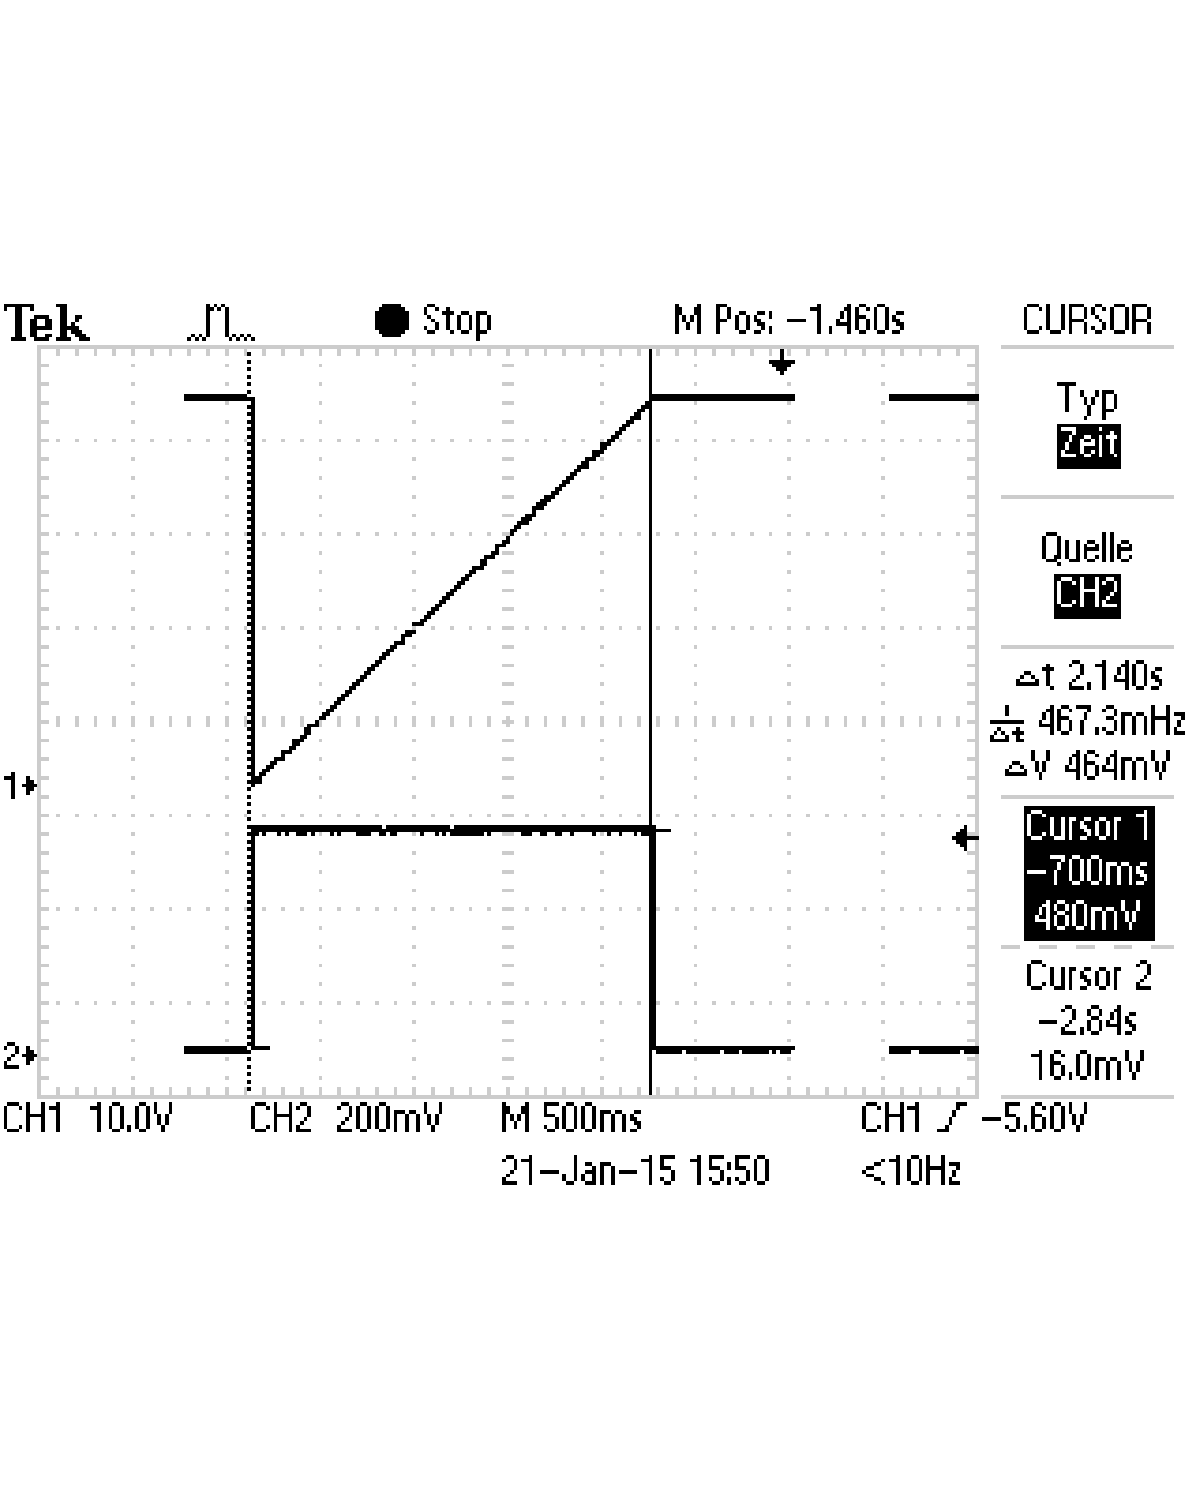
\includegraphics[trim = 0mm 50mm 0mm 50mm, clip, scale = 0.4]{2_1_2V.pdf}
  	\caption[Aufnahme der Ausgangs- und Komparatorspannung für eine Eingangssignal von 2V]{Aufnahme der Ausgangs- und Komparatorspannung für eine Eingangssignal von 2V} 
  \label{fig:2_1_2V}
\end{figure}

In Abbildung \ref{fig:2_1_4V} ist der Verlauf der Referenzspannung und der Komparatorspannung für die Umwandlung eines 4V Signals in ein digitales Signal dargestellt. An der Zeitauflösung ist zu sehen, das dass Umwandeln kürzer dauert als das Umwandeln des 2V Signals.

\begin{figure}[H]
  \centering 	
    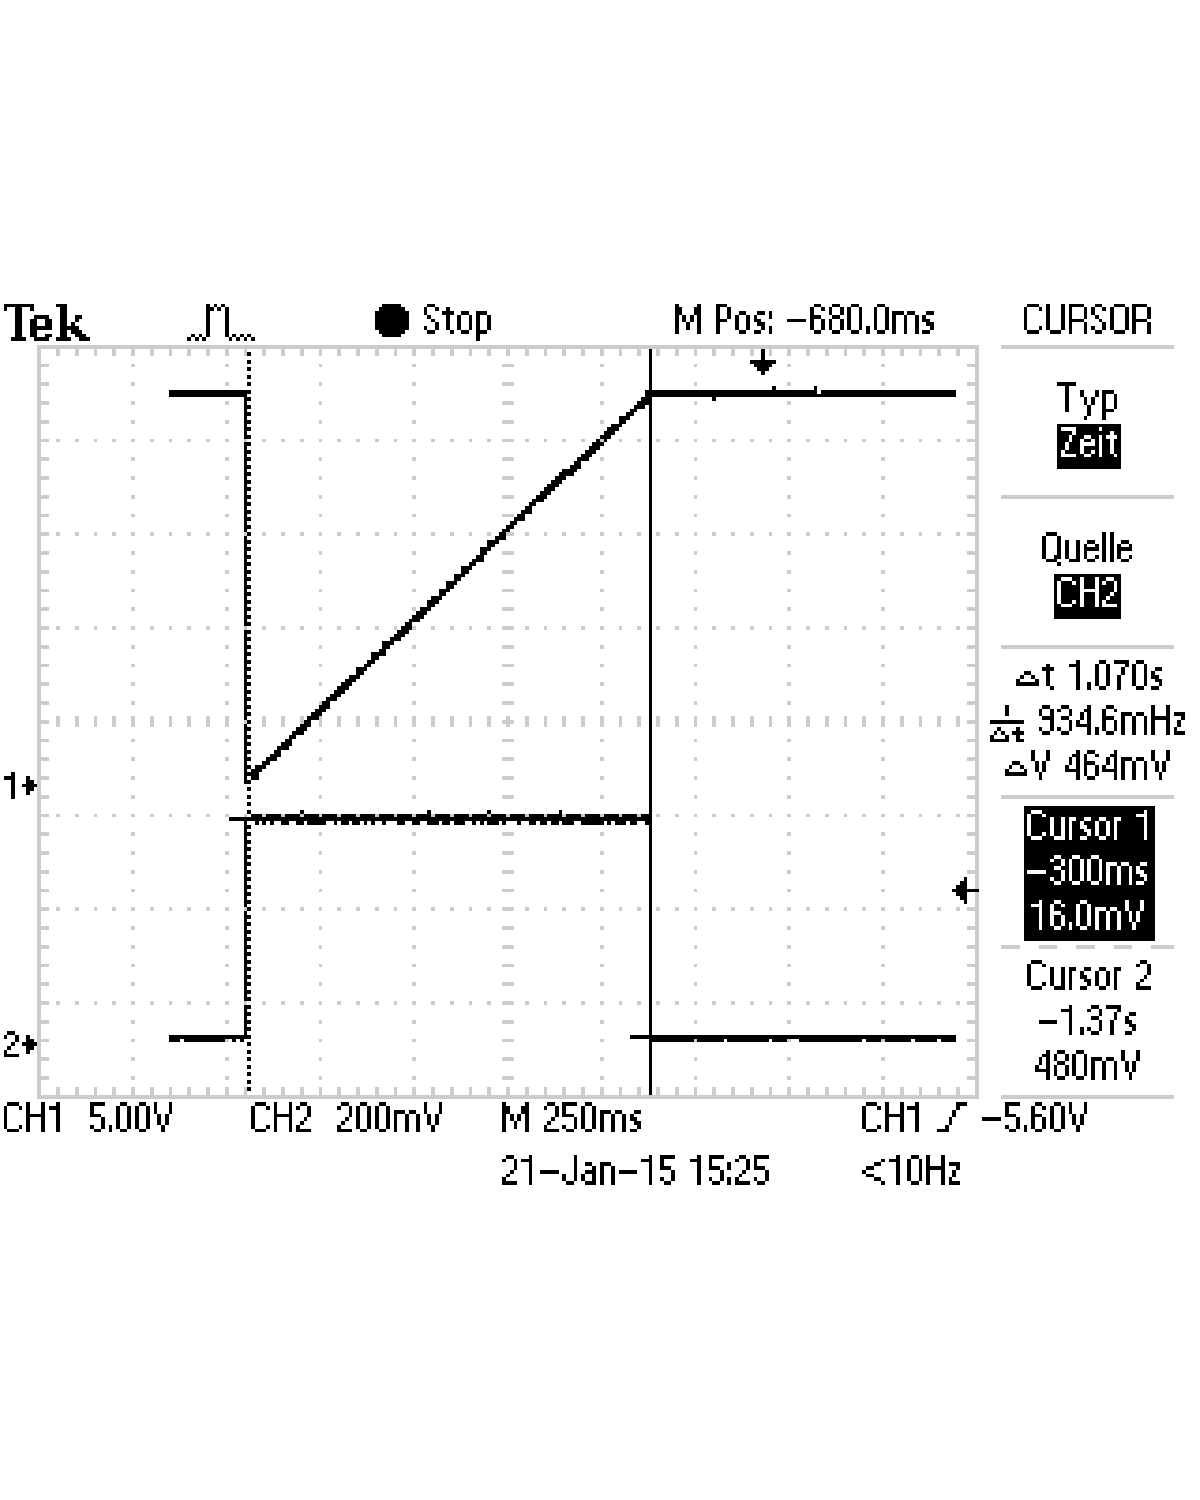
\includegraphics[trim = 0mm 50mm 0mm 50mm, clip, scale = 0.4]{2_1_4V.pdf}
  	\caption[Aufnahme der Ausgangs- und Komparatorspannung für ein Eingangssignal von 4V]{Aufnahme der Ausgangs- und Komparatorspannung für ein Eingangssignal von 4V} 
  \label{fig:2_1_4V}
\end{figure}

Bei der Umwandlung eines 2V Signals mit dem Approximationsverfahren ergab sich der Verlauf in Abbildung \ref{fig:2_2_2V}. Die untere Kurve ist das Signal des Komparators und die obere Kurve ist das Signal der Steuereinheit.

\begin{figure}[H]
  \centering 	
    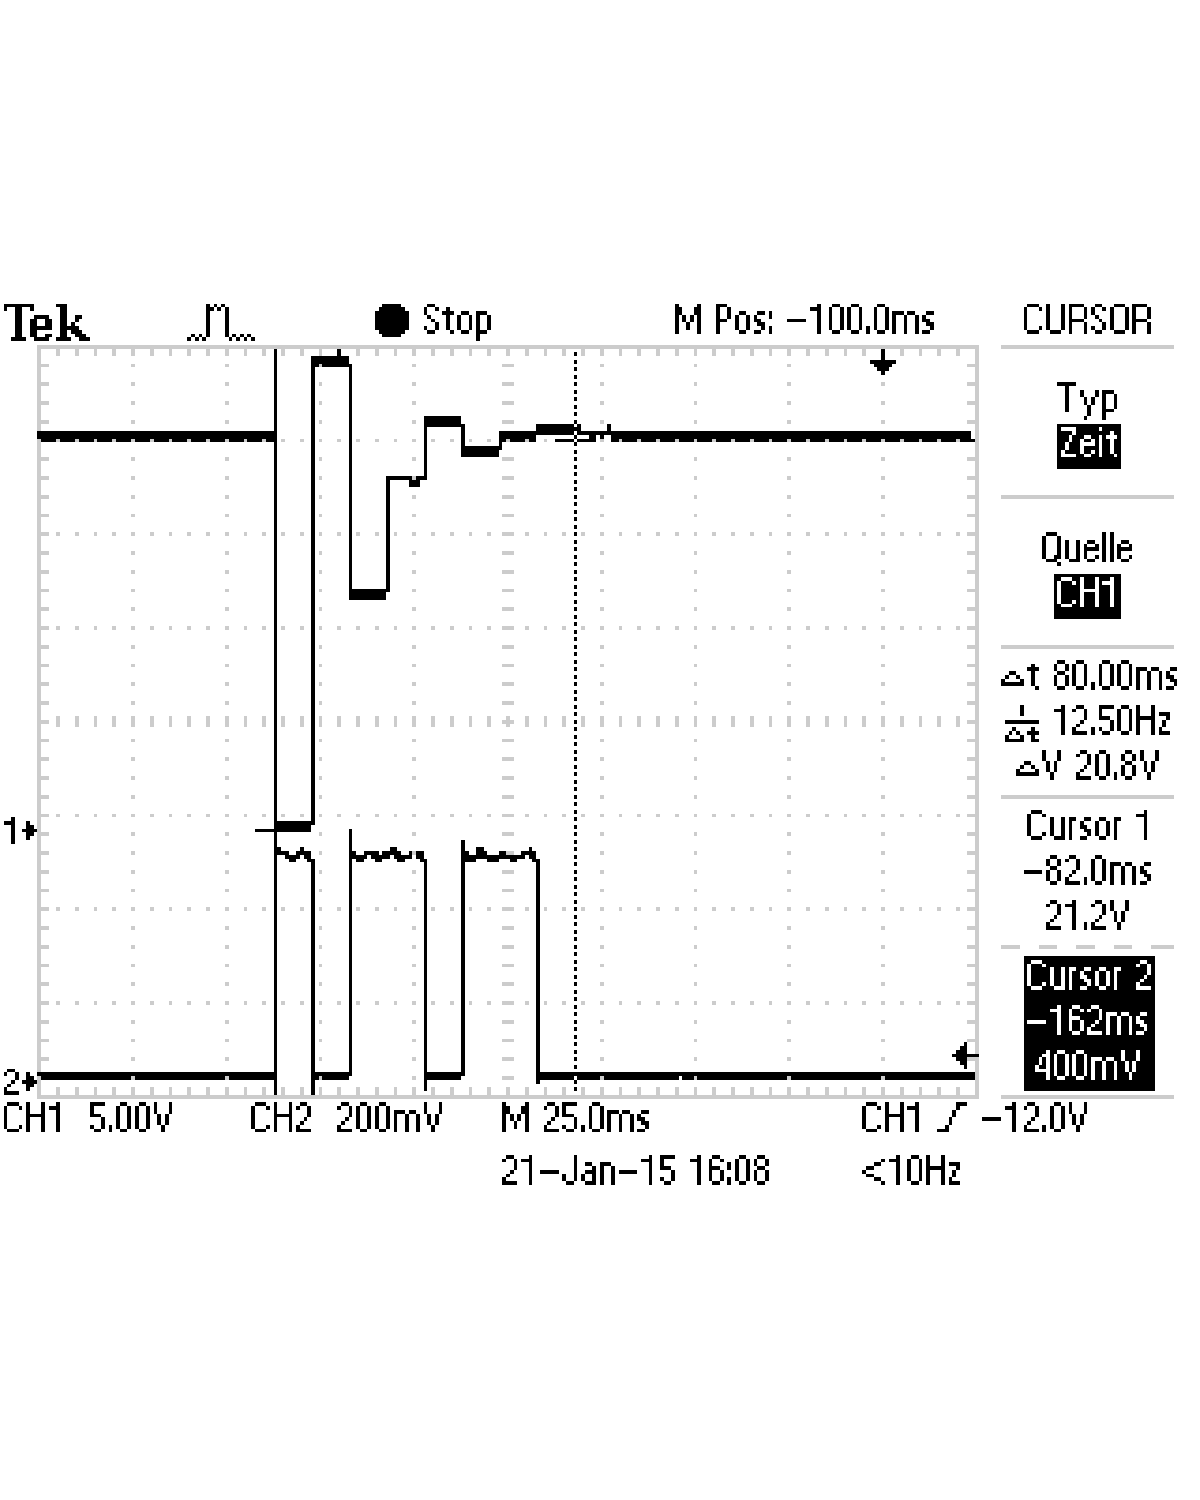
\includegraphics[trim = 0mm 50mm 0mm 50mm, clip, scale = 0.4]{2_2_2V.pdf}
  	\caption[Aufnahme der Ausgangs- und Komparatorspannung für ein Eingangssignal von 2V]{Aufnahme der Ausgangs- und Komparatorspannung für ein Eingangssignal von 2V} 
  \label{fig:2_2_2V}
\end{figure}

Die Umwandelung eines 4V Signals ist in Abbildung \ref{fig:2_2_4V} zu sehen. Die benötigte Zeit dafür ist etwas länger, als beim Umwandeln des 2V Signals. Die Zeitdifferenz lässt sich mit leider nicht erklären, da nicht bekannt ist, wie intern die Routine der Steuereinheit geschrieben ist.

\begin{figure}[H]
  \centering 	
    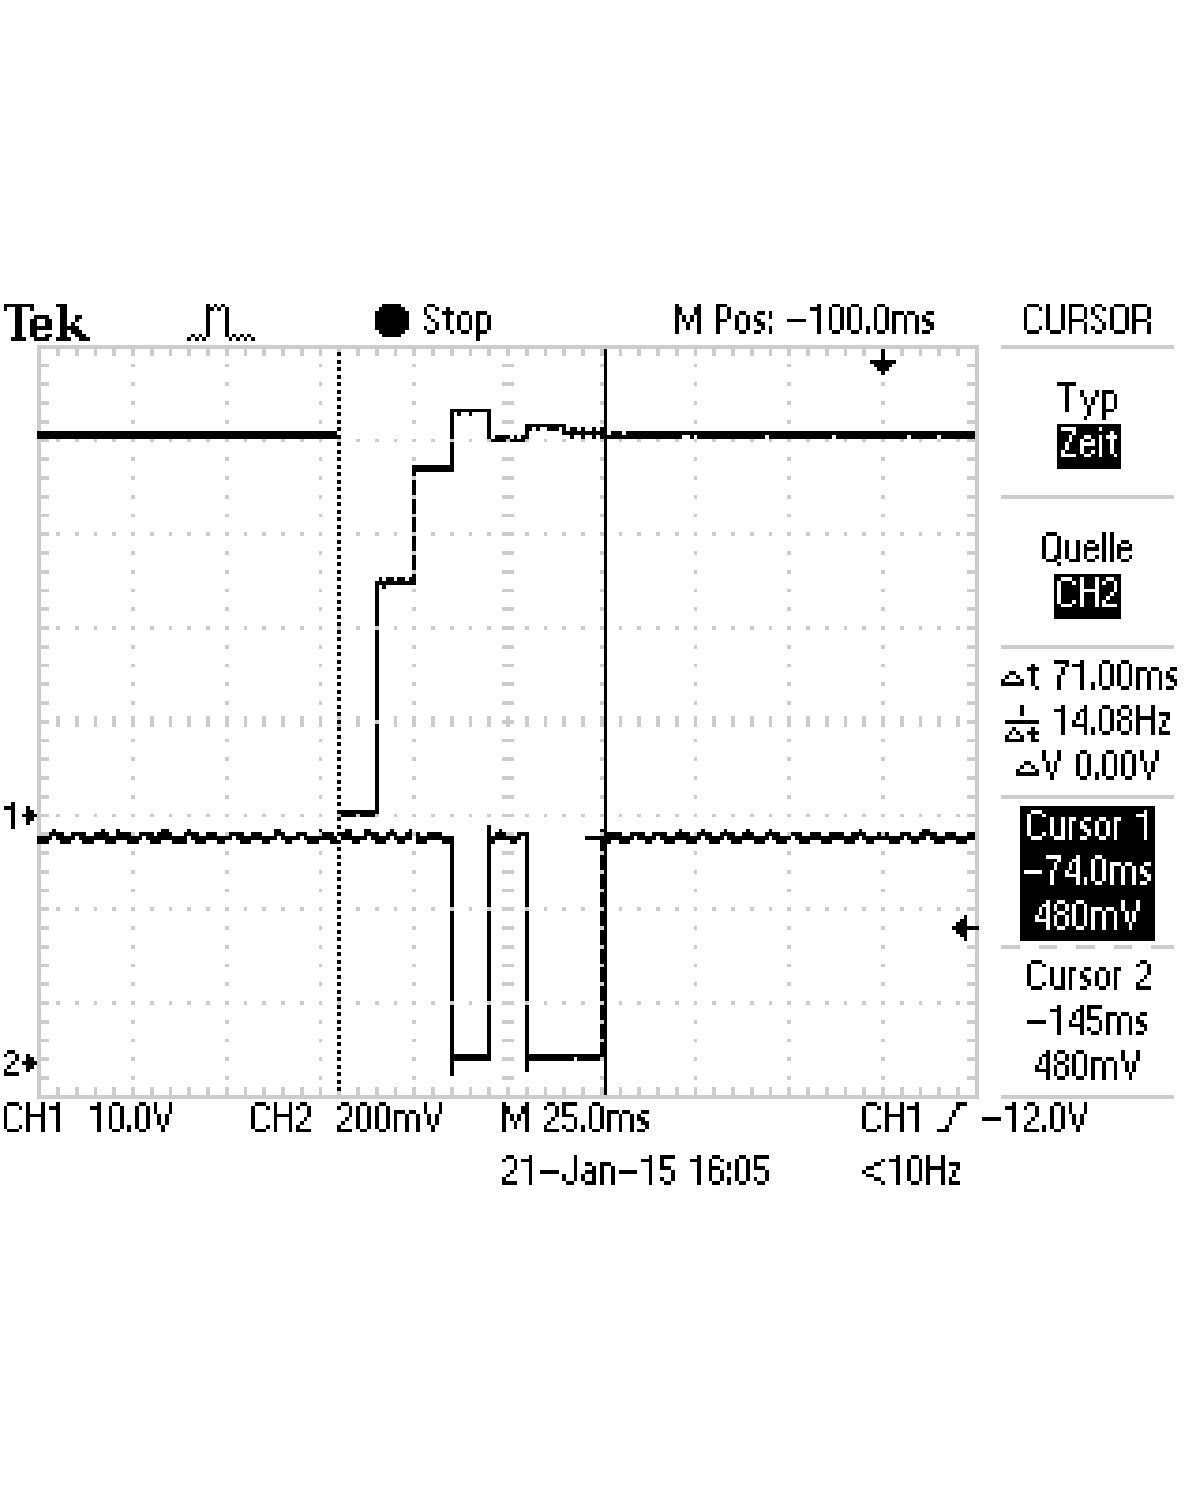
\includegraphics[trim = 0mm 50mm 0mm 50mm, clip, scale = 0.4]{2_2_4V.pdf}
  	\caption[Aufnahme der Ausgangs- und Komparatorspannung für ein Eingangssignal von 4V]{Aufnahme der Ausgangs- und Komparatorspannung für ein Eingangssignal von 4V} 
  \label{fig:2_2_4V}
\end{figure}


Aus den Abbildung \ref{fig:2_1_2V} bis \ref{fig:2_2_4V} kann die jeweils benötigte Zeit abgelesen werden. Daraus lassen sich die Unterschiede in der Dauer der Umwandlung berechnen. Für das Umwandeln des 2V Signals ergibt sich eine Zeitdifferenz von 2,069s und für das Umwandeln des 4V Signals eine Differenz von 1s.

Die Hexadezimal und Dezimalzahlen so wie die daraus bestimmten Bitmuster und die abgelesenen Bitmuster sind in Tabelle \ref{tab:zaehl} für das Zählverfahren und in Tabelle \ref{tab:approx} für das Approximationsverfahren dargestellt. Die aus den Hexadezimalwerten bestimmten Bitmuster stimmen mit den abgelesenen Bitmustern überein.

Die maximal messbare Spannung liegt bei 5V, da die maximale Ausgangsspannung des DACs 5V beträgt.

Beim Steuern des Approximationsverfahren mit einem Taster war zu erkennen, das nach jedem Drücken des Tasters die Änderung der Referenzspannung kleiner wurde.

\subsubsection*{Diskussion}
%(immer) die gemessenen werte und die bestimmten werte über die messfehler mit literaturwerten oder untereinander vergleichen
%in welchem fehlerintervall des messwertes liegt der literaturwert oder der vergleichswert?
%wie ist der relative anteil des fehlers am messwert und damit die qualität unserer messung?
%in einem satz erklären, wie gut unser fehler und damit unsere messung ist
%kurz erläutern, wie systematische fehler unsere messung beeinflusst haben könnten
%(wichtig) zum schluss ansprechen, in wie weit die ergebnisse mit der theoretischen vorhersage übereinstimmen
%--------------------------------------------------------------------------------------------
%falls tabellen mit den messwerten zu lang werden, kann die section mit den messwerten auch hinter der diskussion angefügt bzw. eine section mit dem anhang eingefügt werden.
%1-----------------------------------------------1

In diesem Versuchabschnitt wurden zwei Typen von ADCs untersucht, einer mit Zählverfahren und einer mit Approximationsverfahren. Dabei wurden insbesondere die Dauer der Umwandelung des Signals untersucht. Der ADC mit Approximationsverfahren ist dabei wesentlich schneller, als der ADC mit Zählverfahren. Für die Umwandlung eines 2V Signals benötigt der ADC mit Zählverfahren 2,069s länger als der ADC mit Approximationsverfahren. Beim Umwandeln eines 4V Signals betrug die Zeitdifferenz zwischen Zähl- und Approximationsverfahren \unit[1]{s}. 




\section{Zeit- und Frequenzmessung}
%kurz das ziel dieses versuchsteiles ansprechen, damit keine zwei überschriften direkt übereinander stehen!
%bei schwierigeren versuchen kann auch der theoretische hintergrund erläutert werden. (mit formeln, herleitungen und erklärungen)

In diesem Versuchsabschnitt werden eine Stoppuhr und ein Frequenzzähler gebaut.

\subsection{Bau einer Stoppuhr}
%kurz das ziel dieses versuchsteiles ansprechen, damit keine zwei überschriften direkt übereinander stehen!
%bei schwierigeren versuchen kann auch der theoretische hintergrund erläutert werden. (mit formeln, herleitungen und erklärungen)

In diesem Versuchsteil wird eine Stoppuhr gebaut, welche mit \unit[1]{MHz} getaktet ist.

\subsubsection*{Verwendete Geräte}
%(immer) eine skizze oder ein foto einfügen, die geräte/materialien !nummerieren! und z.b. eine legende dazu schreiben, besser wäre es das ganze in einem Fließtext gut zu beschreiben.
%falls am anfang des versuches nicht klar ist, was alles verwendet wird, wenn möglich erst am ende ein großes foto von den verwendeten materialien machen!\\

Es werden ein Taktzähler Typ 4040, ein Kondensator, Widerstände, ein NAND-Gatter, LEDs, eine Spannungsquelle und das Breadboard verwendet.

\subsubsection*{Versuchsaufbau}
%skizze zum versuchsaufbau (oder foto) einfügen,   es muss erklärt werden wie das ganze funktioniert und welche speziellen einstellungen verwendet wurden (z.b. welche knöpfe an den geräten für die messung verdreht wurden)

Schaltplan zum Aufbau der Stoppuhr.

\begin{figure}[H] 
  \centering 	
    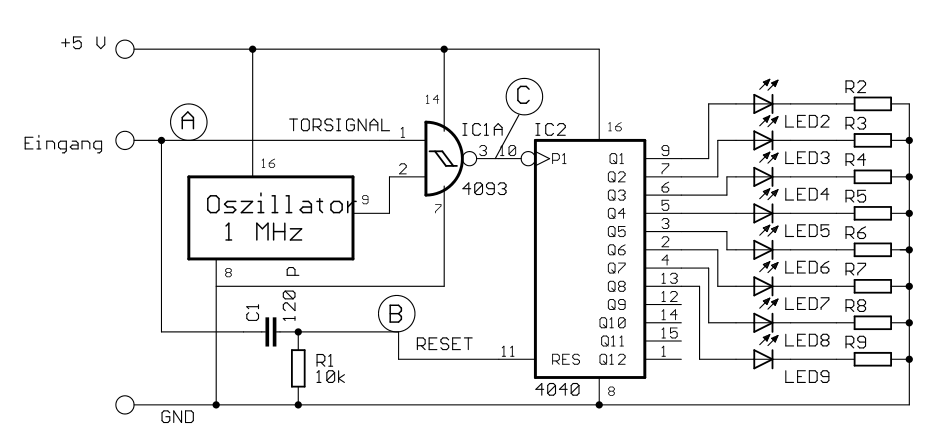
\includegraphics[ scale = 0.4]{auf_5.png}
  	\caption[Schaltplan der Stoppuhr]{Schaltplan der Stoppuhr\footnotemark}
  \label{fig:auf_3}
\end{figure}
\footnotetext{Abbildung entnommen von http://www.atlas.uni-wuppertal.de/$\sim$kind/ep11\_14.pdf am 18.01.2015}

\subsubsection*{Versuchsdurchführung}
%erklären, !was! wir machen, !warum! wir das machen und mit welchem ziel
%(wichtig) präzize erklären, wie bei dem versuch vorgegangen und was gemacht wurde

Nachdem die Schaltung  in Abb. \ref{fig:auf_3}  am Breadboard aufgebaut wurde, wird ein Eingangssignal mit einer Amplitude von 5V (Rechteckpulse mit kurzer Signalbreite und langen Pausen) eingestellt. Die Frequenz des Funktionsgenerators wird so gewählt, das die Maximalzeit, welche mit der Stoppuhr gemessen werden kann, nicht überstiegen wird (8 LEDs und \unit[1]{MHz} Oszillator $\Rightarrow$ f $\gtrsim$ \unit[4]{kHz} bzw. T $\lesssim$ \unit[0,25]{ms}). Danach wird das Bitmuster der LEDs gelesen und umgerechnet. Die Impulse des Funktionsgenerators werden dann mit dem Oszilloskop untersucht um nochmal die Pulsdauer zu bestimmen, welche mit den gemessenen Werten verglichen werden soll. Für das Durchlaufen der zwölf Bits (8 LEDs) werden 4 Millisekunden benötigt.

\subsubsection*{Auswertung}
%zuerst !alle! errechneten werte entweder in ganzen sätzen aufzählen, oder in tabellen (übersichtlicher) dargestellen, sowie auf die verwendeten formeln verweisen (die referenzierung der formel kann in der überschrift stehen)
%kurz erwähnen (vor der tabelle), warum wir das ganze ausrechnen bzw. was wir dort ausrechnen
%danach histogramme und plots erstellen, wobei wenn möglich funktionen durch die plots gelegt werden (zur not können auch splines benutzt werden, was aber angegeben werden muss)
%bei fits immer die funktion und das reduzierte chiquadrat mit angegeben, wobei auf verständlichkeit beim entziffern der zehnerpotenzen geachtet werden muss z.b. f(x)=(wert+-fehler)\cdot10^{irgendeine zahl}\cdot x + (wert+-fehler)\cdot10^{irgendeine zahl}
%bei jedem fit erklären, nach welchem zusammenhang gefittet wurde und warum!
%bei plots darauf achten, dass die achsenbeschriftung (auch die tics) die richtige größe haben und die legende im plot nicht die messwerte verdeckt
%kurz die aufgabenstellung abhandeln
%2-----------------------------------------------2
In Abbildung \ref{fig:impulse} sind die Aufnahmen der Impulse des Funktionsgenerators mit dem Oszilloskop dargestellt.
\begin{figure}[H]
\centering
\begin{subfigure}[b]{0.45\textwidth}
\centering
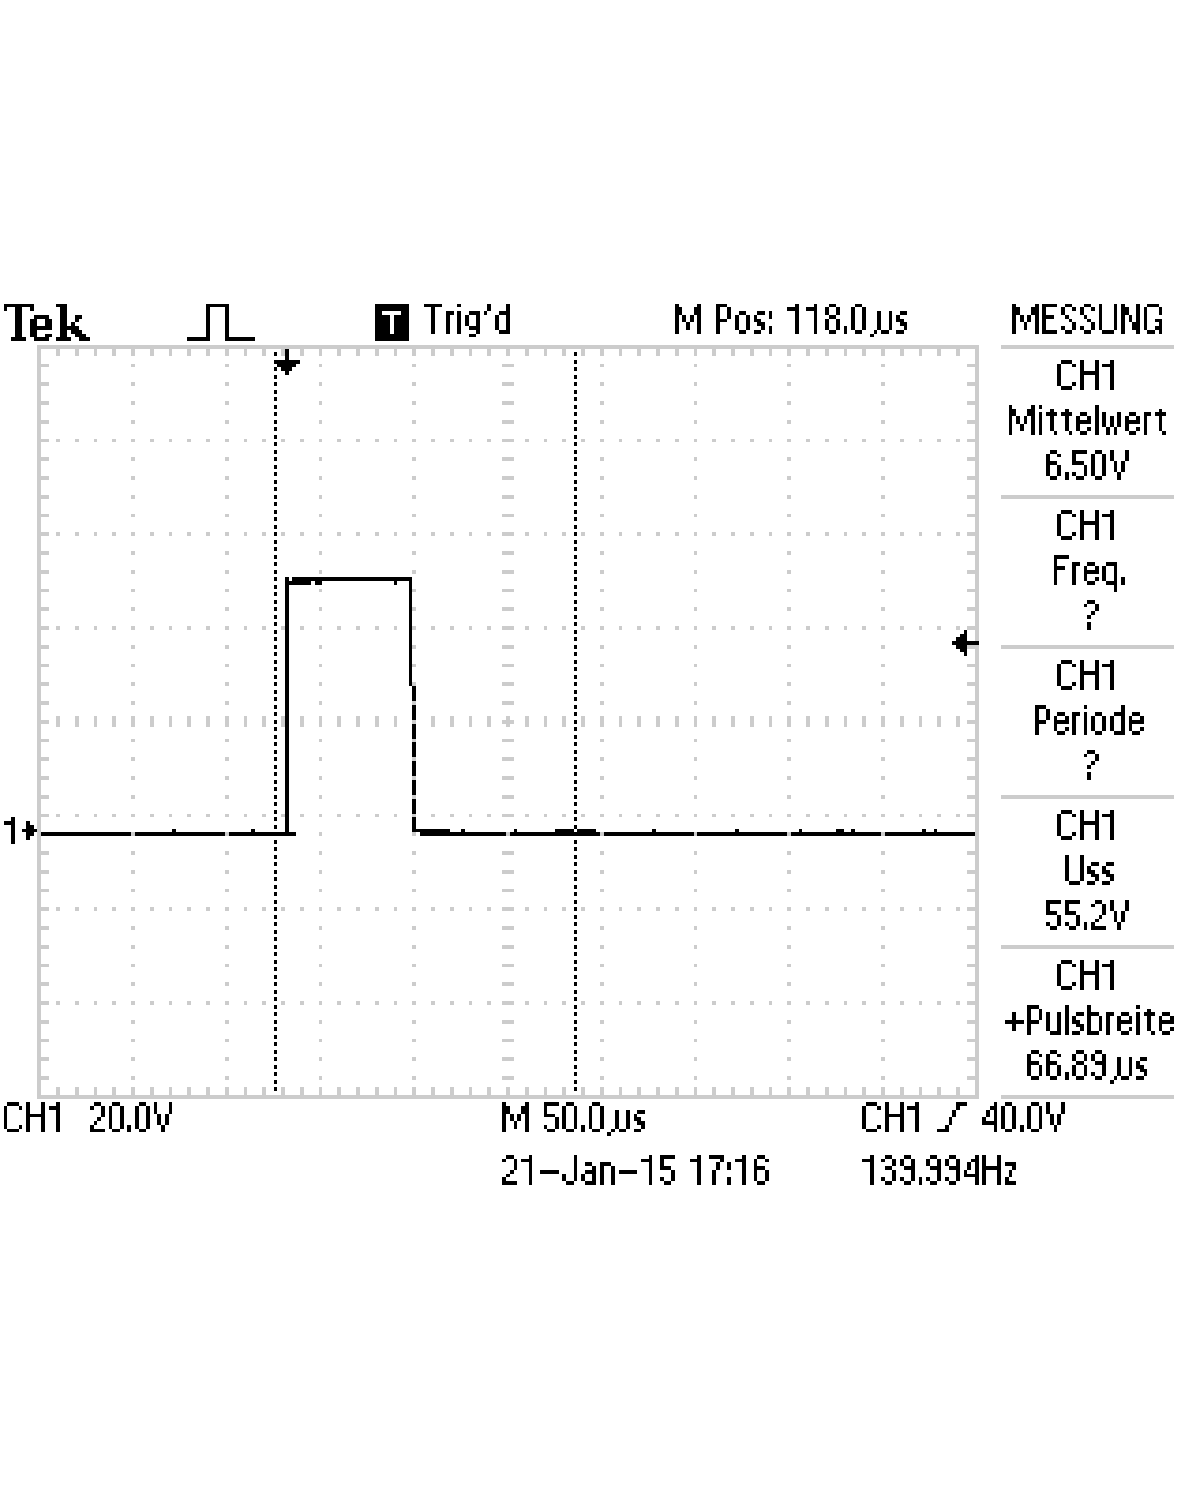
\includegraphics[scale=0.4]{3_1_67.pdf}
\caption[Aufnahme des 2. Impulses mit dem Oszilloskop]{Aufnahme des zweiten Impulses mit dem Oszilloskop}
\end{subfigure}
\hfill
\begin{subfigure}[b]{0.45\textwidth}
\centering
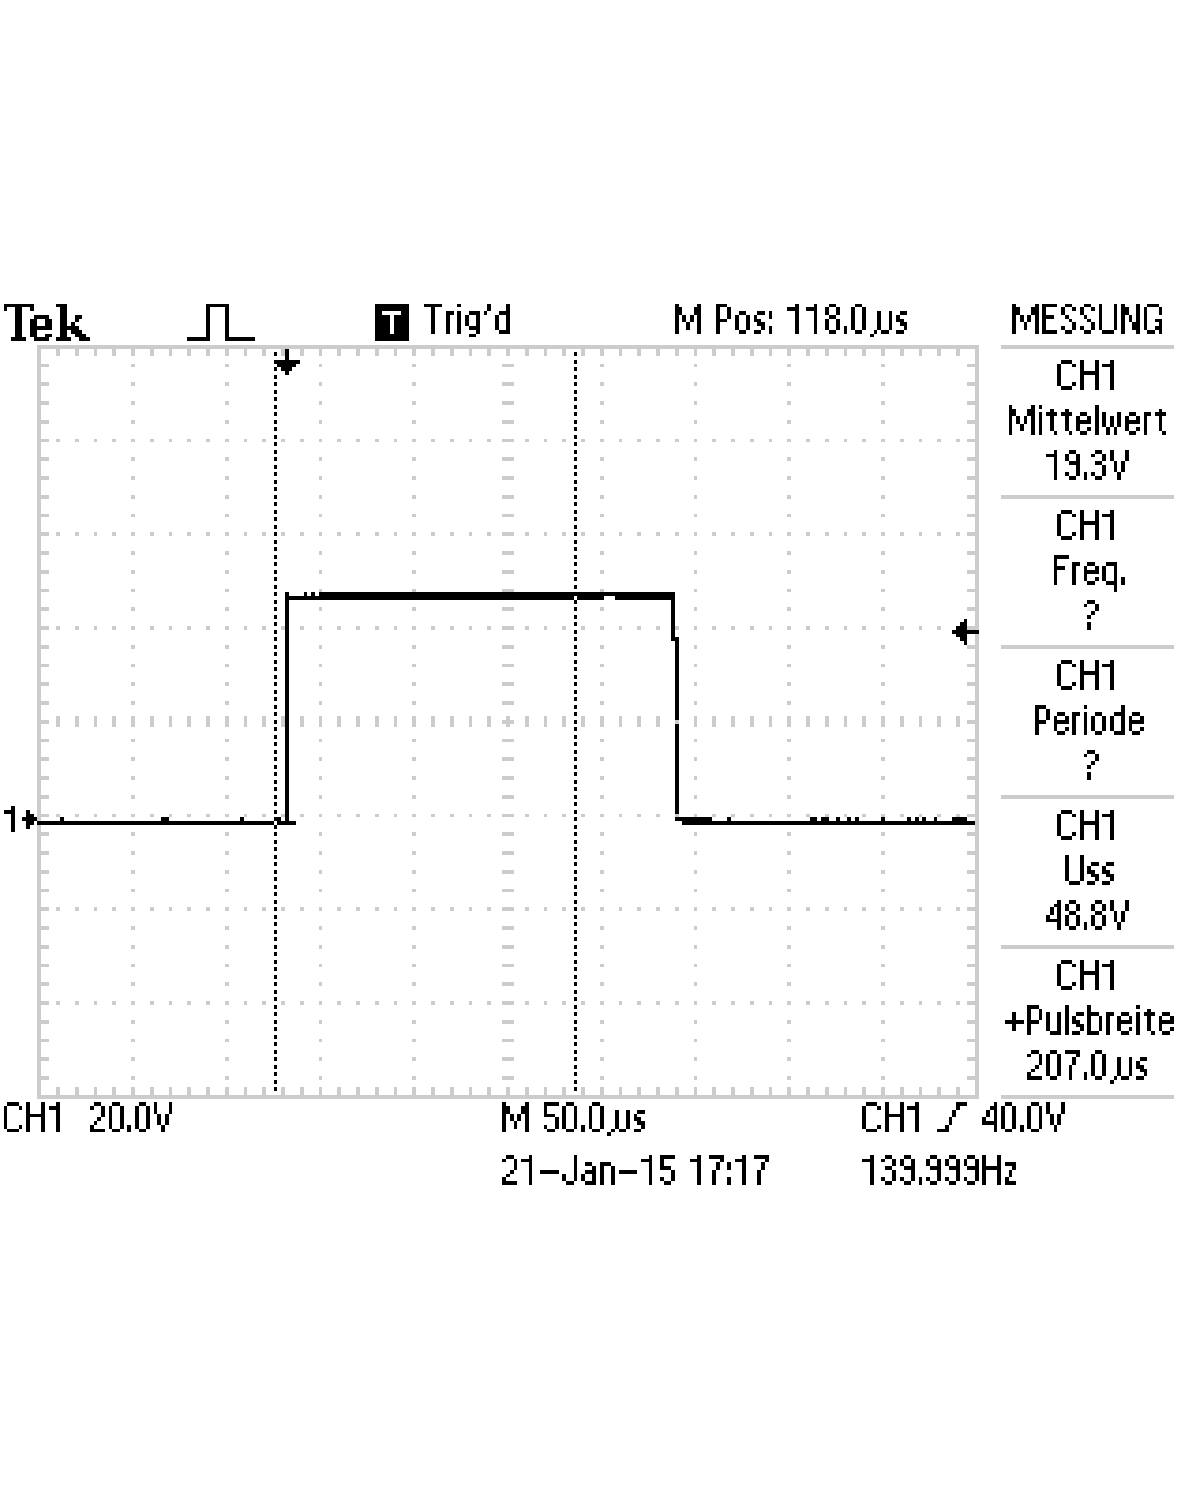
\includegraphics[scale=0.4]{3_1_207.pdf}
\caption[Aufnahme des 3. Impulses mit dem Oszilloskop]{Aufnahme des dritten Impulses mit dem Oszilloskop}
\end{subfigure}
\caption[Aufnahme der Impulse]{Aufnahme der Impulse}
\label{fig:impulse}
\end{figure}
In Tabelle \ref{tab:span} sind die eingestellten Pulsbreiten und die dazu an den LEDs abgelesenen Binärmuster dargestellt. Der Impuls für das erste Signal wurde ebenso mit dem Oszilloskop gemessen, aber nicht abgespeichert. Deshalb sind in Abb. \ref{fig:impulse} die Impulse für die zweite und dritte Messung zu sehen.
\begin{table}[H]
\begin{center}
\begin{tabular}{|r|l|l|}
	\hline
	\multicolumn{1}{|l|}{Pulsbreite/{\unit{$\mu$s}}} & Binärmuster & Binär $\rightarrow$ Dezimal\\ \hline\hline
	                                           19,05 & 0b00010011  & 19\\ \hline
	                                           66,89 & 0b01000011  & 67\\ \hline
	                                           207,1 & 0b11001111  & 207\\ \hline
\end{tabular}
\end{center}
\caption{Bitmuster in Abhängigkeit der Frequenz}
\label{tab:span}
\end{table}
Um die Impulsdauern mit dem Oszilloskop zu messen, wurde die Funktion "`measure"' verwendet. Sobald die Impulsdauer größer ist als die Maximalzeit der Stoppuhr, zählt diese wieder binär von 0 hoch, sodass z.B. anstatt einer 260 bei \unit[260]{$\mu$s} Impulsdauer und 8 LEDs eine binäre 4 angezeigt wird. Durch das binäre Hochzählen bis 260 entsteht dabei ein Hintergrundflackern bei allen nicht dauerhaft aufleuchtenden LEDs. Die Intensität des Hintergrundflackerns ist abhängig vom Impuls-Pausen-Verhältnis und nimmt ab, falls die Impulsbreiten klein gegen die Länge der Pausen sind. Die Impulsbreiten sollten daher möglichst klein gewählt werden. Zwischen NAND-Gatter und Zähler ist das invertierte Signal des Oszillators zu sehen, solange am Eingang Spannung anliegt. 

\subsection{Bau eines Frequenzzählers}
%kurz das ziel dieses versuchsteiles ansprechen, damit keine zwei überschriften direkt übereinander stehen!
%bei schwierigeren versuchen kann auch der theoretische hintergrund erläutert werden. (mit formeln, herleitungen und erklärungen)
In diesem Versuchsteil wird die Stoppuhr in einen Frequenzzähler umgebaut, welcher für einen vorgegebenen Zeitraum die Anzahl der am Eingang eintreffenden Impulse zählen soll.
\subsubsection*{Verwendete Geräte}
%(immer) eine skizze oder ein foto einfügen, die geräte/materialien !nummerieren! und z.b. eine legende dazu schreiben, besser wäre es das ganze in einem Fließtext gut zu beschreiben.
%falls am anfang des versuches nicht klar ist, was alles verwendet wird, wenn möglich erst am ende ein großes foto von den verwendeten materialien machen!\\
Es werden drei Taktzähler Typ 4040, ein Kondensator, zwei Widerstände, ein NAND-Gatter, LEDs, ein Oszillator, einen HAMEG-Funktionsgenerator und eine Spannungsquelle verwendet.
\subsubsection*{Versuchsaufbau}
%skizze zum versuchsaufbau (oder foto) einfügen,   es muss erklärt werden wie das ganze funktioniert und welche speziellen einstellungen verwendet wurden (z.b. welche knöpfe an den geräten für die messung verdreht wurden)
Schaltplan zum Aufbau eines Frequenzzählers.
\begin{figure}[H] 
  \centering 	
    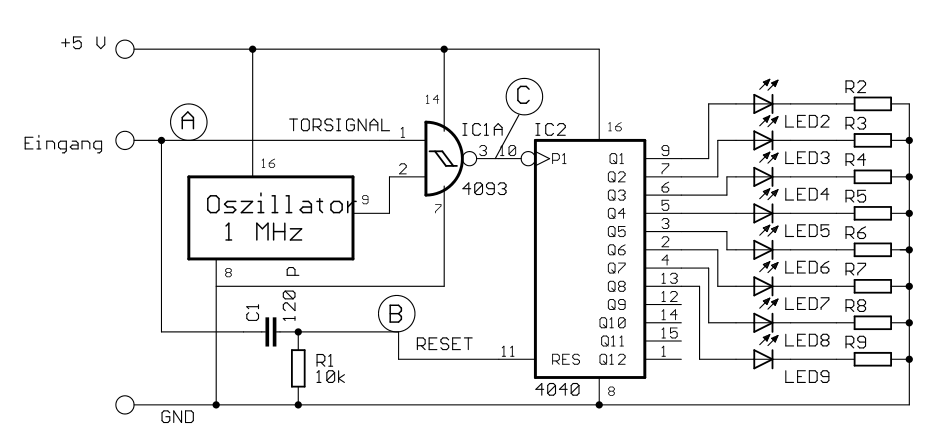
\includegraphics[ scale = 0.4]{auf_5.png}
  	\caption[Schaltplan des Frequenzzählers]{Schaltplan des Frequenzzählers\footnotemark}
  \label{fig:auf_3_2}
\end{figure}
\footnotetext{Abbildung entnommen von http://www.atlas.uni-wuppertal.de/$\sim$kind/ep11\_14.pdf am 18.01.2015}
\subsubsection*{Versuchsdurchführung}
%erklären, !was! wir machen, !warum! wir das machen und mit welchem ziel
%(wichtig) präzize erklären, wie bei dem versuch vorgegangen und was gemacht wurde
Die Stoppuhr wird zum Frequenzzähler umgebaut, indem das Torsignal vom Oszillator gewonnen wird. Zwischen Oszillator und NAND-Baustein werden zwei Zähler geschaltet, welche die Frequenz des Oszillators durch $2^{22}$ teilen (siehe Schaltung \ref{fig:auf_3_2}). Die Torzeit beträgt jetzt eine Sekunde (\unit[0,5]{Hz}), da der Oszillator mit einer Frequenz von \unit[2,09715]{MHz} arbeitet. Sobald die Schaltung aufgebaut wurde, wird mit dem Oszilloskop überprüft ob das Eingangssignal zwischen 0 und \unit[5]{V} liegt und eine Spannung von \unit[5]{V} eingestellt. Dann wird die Frequenz der Ausgangsimpulse des Funktionsgenerators gemessen. Die maximal Messbare Frequenz liegt bei genau \unit[4,095]{kHz}, falls 12 LEDs verwendet werden (\unit[255]{Hz} für 8 LEDs), daher muss das Eingangssignal passend gewählt werden. Zum Schluss wird der Messwert mit der Anzeige am Funktionsgenerator verglichen.
\subsubsection*{Auswertung}
%zuerst !alle! errechneten werte entweder in ganzen sätzen aufzählen, oder in tabellen (übersichtlicher) dargestellen, sowie auf die verwendeten formeln verweisen (die referenzierung der formel kann in der überschrift stehen)
%kurz erwähnen (vor der tabelle), warum wir das ganze ausrechnen bzw. was wir dort ausrechnen
%danach histogramme und plots erstellen, wobei wenn möglich funktionen durch die plots gelegt werden (zur not können auch splines benutzt werden, was aber angegeben werden muss)
%bei fits immer die funktion und das reduzierte chiquadrat mit angegeben, wobei auf verständlichkeit beim entziffern der zehnerpotenzen geachtet werden muss z.b. f(x)=(wert+-fehler)\cdot10^{irgendeine zahl}\cdot x + (wert+-fehler)\cdot10^{irgendeine zahl}
%bei jedem fit erklären, nach welchem zusammenhang gefittet wurde und warum!
%bei plots darauf achten, dass die achsenbeschriftung (auch die tics) die richtige größe haben und die legende im plot nicht die messwerte verdeckt
%kurz die aufgabenstellung abhandeln
%2-----------------------------------------------2
In Tabelle \ref{tab:frequ} werden die am Oszilloskop abgelesenen Frequenzen des Funktionsgenerators und die an den LEDs angezeigten Frequenzen in Binärcode sowie im Dezimalsystem dargestellt.
\begin{table}[H]
\begin{center}
\begin{tabular}{|r|l|l|}
	\hline
	\multicolumn{1}{|l|}{Frequenz/Hz} & Binärmuster & Binär $\rightarrow$ Dezimal \\ \hline\hline
	                              140 & 0b10001100  & 140                         \\ \hline
	                               86 & 0b01010110  & 86                          \\ \hline
	                               32 & 0b00100000  & 32                          \\ \hline
	                                8 & 0b00001000  & 8                           \\ \hline
\end{tabular}
\end{center}
\caption{Bitmuster in Abhängigkeit der Frequenz}
\label{tab:frequ}
\end{table}
Für den Frequenzzähler wurden keine zusätzlichen Aufnahmen der Impulse getätigt, denn man kann die Übereinstimmung der eingestellten Frequenzen mit den an den LEDs angezeigten Frequenzen klar erkennen. Es wurden 8 LEDs verwendet.



\subsubsection*{Diskussion}
%(immer) die gemessenen werte und die bestimmten werte über die messfehler mit literaturwerten oder untereinander vergleichen
%in welchem fehlerintervall des messwertes liegt der literaturwert oder der vergleichswert?
%wie ist der relative anteil des fehlers am messwert und damit die qualität unserer messung?
%in einem satz erklären, wie gut unser fehler und damit unsere messung ist
%kurz erläutern, wie systematische fehler unsere messung beeinflusst haben könnten
%(wichtig) zum schluss ansprechen, in wie weit die ergebnisse mit der theoretischen vorhersage übereinstimmen
%--------------------------------------------------------------------------------------------
%falls tabellen mit den messwerten zu lang werden, kann die section mit den messwerten auch hinter der diskussion angefügt bzw. eine section mit dem anhang eingefügt werden
%1-----------------------------------------------1
Die in diesem Versuchsabschnitt untersuchten Schaltungen zeigten das erwartete Verhalten. Der Frequenzzähler sowie die Stoppuhr konnte die verwendeten Impulsfrequenzen/dauern mit den LEDs gut wiedergeben, da alle Frequenzen/Impulsdauern im Bereich der Genauigkeit des Frequenzzählers/der Stoppuhr korrekt angezeigt wurden.

\section{Fazit}
%im fazit nochmal alles zusammenfassen und den verlauf der messung abschätzen
%gravierende sytematische probleme bei den messungen nochmal betonen und die wertigkeit unserer ergebnisse einordnen

In diesem Versuch wurde die Erfassung von Daten mit Computern/Mikrocontrollern untersucht. Dabei wurde das Umwandeln seinen digitalen Signals in eine analoges und das Umwandeln eines analogen in ein digitales Signal untersucht. Bei allen durchgeführten Versuchen in diesen Abschnitten wurden die erwarteten Ergebnisse erzielt. Dabei zeigte sich, dass die Umwandelung eines analogen Signals in ein digitales mit dem Approximationsverfahren deutlich schneller geht als mit dem Zählerverfahren. Im letzten Versuchsabschnitt sollten noch eine Stoppuhr und ein Frequenzzähler gebaut werden. Diese ließen funktionierten wie erwartet und es konnte die Theorie bestätigt werden.

\end{document}

